\documentclass[a4paper,12pt]{article}

% ==============================================================================
% GÓI HỖ TRỢ TIẾNG VIỆT VÀ ĐỊNH DẠNG TRANG
% ==============================================================================
\usepackage[utf8]{inputenc}
\usepackage{vntex}
\usepackage{a4wide}
\usepackage{geometry}
\geometry{a4paper, margin=1in, headheight=40pt}
\usepackage{setspace}
\onehalfspacing
\usepackage{enumitem}
% ==============================================================================
% TOÁN HỌC, BẢNG BIỂU VÀ HÌNH ẢNH
% ==============================================================================
\usepackage{amsmath,amssymb,amsfonts,bm}
\usepackage{float}
\usepackage{graphicx}
\usepackage{subcaption}
\usepackage{caption}
\usepackage{booktabs}
\usepackage{tabularx}
\usepackage{multirow}
\usepackage{multicol}
\usepackage{array}
\usepackage{lastpage}
\usepackage{fancyhdr}

% Tăng khoảng cách dòng trong bảng để không bị dính nét kẻ khi dùng lưới ô
\renewcommand{\arraystretch}{1.25}

% ==============================================================================
% ĐỊNH DẠNG CODE PYTHON & THUẬT TOÁN (IOT GATEWAY)
% ==============================================================================
\usepackage{xcolor}
\usepackage{listings}
\lstset{
    basicstyle=\ttfamily\small,
    keywordstyle=\color{blue}\bfseries,
    commentstyle=\color{green!60!black},
    stringstyle=\color{red},
    breaklines=true,
    frame=single,
    columns=fullflexible,
    numbers=left,
    numberstyle=\tiny,
    stepnumber=1,
    numbersep=5pt,
    language=Python
}

% ==============================================================================
% TỪ ĐIỂN TỪ VIẾT TẮT & KÝ HIỆU (GLOSSARIES - CHUYÊN NGÀNH IOT & HỆ THỐNG)
% ==============================================================================
\usepackage[
    sort=none,
    abbreviations,
    symbols,
    stylemods,style=list,
    nogroupskip, nonumberlist, nomain
]{glossaries-extra}

\setabbreviationstyle{long-short}
\newabbreviation{iot}{IoT}{Internet of Things}
\newabbreviation{mqtt}{MQTT}{Message Queuing Telemetry Transport}
\newabbreviation{rbac}{RBAC}{Role-Based Access Control}
\newabbreviation{srs}{SRS}{Software Requirements Specification}
\newabbreviation{uc}{UC}{Use Case}
\newabbreviation{fr}{FR}{Functional Requirement}
\newabbreviation{nfr}{NFR}{Non-Functional Requirement}
\newabbreviation{api}{API}{Application Programming Interface}
\newabbreviation{ui}{UI}{User Interface}
\newabbreviation{httt}{HTTT}{Hệ thống thông tin}

% ==============================================================================
% TÀI LIỆU THAM KHẢO & LIÊN KẾT
% ==============================================================================
\usepackage[colorlinks]{hyperref}
\hypersetup{urlcolor=blue, linkcolor=black, citecolor=black}
\usepackage{biblatex}
\addbibresource{citations.bib}

% ==============================================================================
% CẤU HÌNH TIÊU ĐỀ ĐẦU TRANG & CHÂN TRANG (HEADER / FOOTER)
% ==============================================================================
\captionsetup[table]{name=Bảng}
\captionsetup[figure]{name=Hình}

\pagestyle{fancy}
\fancyhead{}
\fancyhead[L]{
    \begin{tabular}{rl}
        \begin{picture}(25,15)(0,0)
            \put(0,-6){
\includegraphics[width=8mm, height=8mm]{hcmut.png}}
        \end{picture}&
        \begin{tabular}{l}
            \textbf{\ttfamily Trường Đại học Bách Khoa TP. Hồ Chí Minh}\\
            \textbf{\ttfamily Khoa Khoa học và Kỹ thuật Máy tính}
        \end{tabular}   
    \end{tabular}
}
\fancyhead[R]{}
\fancyfoot{}
\fancyfoot[L]{\scriptsize \ttfamily Đồ án: Quản lý Thiết bị Nông trại Thông minh}
\fancyfoot[R]{\scriptsize \ttfamily Trang {\thepage}/\pageref{LastPage}}
\renewcommand{\headrulewidth}{0.3pt}
\renewcommand{\footrulewidth}{0.3pt}

\setcounter{secnumdepth}{4}
\setcounter{tocdepth}{3}

% ==============================================================================
% BẮT ĐẦU TÀI LIỆU
% ==============================================================================
\begin{document}

% ---------------- TRANG BÌA ----------------
\begin{titlepage}
\begin{center}
    ĐẠI HỌC QUỐC GIA TP. HỒ CHÍ MINH \\
    TRƯỜNG ĐẠI HỌC BÁCH KHOA \\
    KHOA KHOA HỌC VÀ KỸ THUẬT MÁY TÍNH
\end{center}

\vspace{0.8cm}

\begin{figure}[h!]
    \centering
    
\includegraphics[width=3cm]{hcmut.png}
\end{figure}

\vspace{0.6cm}

\begin{center}
    \begin{tabular}{c}
        \textbf{\Large BÁO CÁO ĐỒ ÁN ĐA NGÀNH}\\
        ~\\
        \hline
        \\
        \textbf{\Huge XÂY DỰNG ỨNG DỤNG}\\
        \vspace{0.2cm}
        \textbf{\Huge QUẢN LÝ THIẾT BỊ NÔNG TRẠI}\\
        \vspace{0.3cm}
        \textbf{\large (SMART FARM DEVICE MANAGEMENT SYSTEM)}\\
        \\
        \hline
    \end{tabular}
\end{center}

\vspace{0.8cm}

\begin{table}[h]
\centering
    \begin{tabular}{rl}
        \hspace{1.5cm}\textbf{Giảng viên hướng dẫn}: & Trần Thị Quế Nguyệt \\[8pt]
        \textbf{Sinh viên thực hiện}: & Lý Trung Hòa -- 2311097\\
                                       & Nguyễn Miên Phú -- 2312658\\
                                       & Trương Thái Nguyên -- 2312391\\
                                       & Ngô Phương Quang -- 2352967\\[6pt]
        \textbf{Nhóm}: & 4
    \end{tabular}
\end{table}

\vfill

\begin{center}
    {\footnotesize TP. Hồ Chí Minh, Năm 2026}
\end{center}
\end{titlepage}

% ---------------- MỤC LỤC & DANH MỤC ----------------
\pagenumbering{roman}

\tableofcontents
\pagebreak

\printunsrtglossary[type={abbreviations}, title={Danh sách các từ viết tắt}]
\pagebreak

\listoffigures
\addcontentsline{toc}{section}{Danh mục Hình ảnh}
\pagebreak

\listoftables
\addcontentsline{toc}{section}{Danh mục Bảng biểu}
\pagebreak

% ---------------- NỘI DUNG CHÍNH ----------------
\pagenumbering{arabic}

% ==============================================================================
% MỤC 1: GIỚI THIỆU ĐỀ TÀI (INTRODUCTION)
% ==============================================================================
\section{Giới thiệu}

\subsection{Bối cảnh và Tính cấp thiết của đề tài}

Nông nghiệp là ngành kinh tế đóng vai trò trụ cột tại Việt Nam, đặc biệt là các mô hình canh tác cây trồng ngoài trời (Open-field Farm) có giá trị kinh tế cao như cây ăn trái (sầu riêng, thanh long, bưởi tại Đồng bằng sông Cửu Long và Đông Nam Bộ) và cây công nghiệp (cà phê, hồ tiêu tại Tây Nguyên). Tuy nhiên, phương thức canh tác truyền thống trên diện tích đất mở hiện đang đối mặt với những thách thức và rủi ro rất lớn:
\begin{itemize}
    \item \textbf{Khí hậu khắc nghiệt, hạn hán và sốc nhiệt mùa khô:} Hiện tượng biến đổi khí hậu gay gắt dẫn đến các đợt nắng nóng cực đoan (nhiệt độ ngoài trời vượt $38 - 40^\circ\text{C}$) kết hợp độ ẩm không khí xuống thấp, làm gia tăng tốc độ bốc thoát hơi nước của cây trồng, gây cháy đọt, rụng hoa và kiệt sức bộ rễ nếu không được phun sương làm mát tầng tán hoặc cấp nước kịp thời.
    \item \textbf{Tưới tiêu và điều tiết ánh sáng theo cảm tính:} Nông dân thường tưới xả tràn hoặc canh giờ tưới dựa trên mắt nhìn bề mặt đất, dẫn đến lãng phí nguồn nước ngầm quý giá và thất thoát chi phí điện năng. Tương tự, ở các vùng chuyên canh hoa cúc hoặc thanh long, việc canh thời gian chong đèn quang kỳ để kích thích ra hoa trái vụ còn mang tính thủ công, thiếu tự động hóa.
    \item \textbf{Khan hiếm nhân công và khó khăn quản lý phân tán:} Với quy mô nông trại rộng nhiều hecta chia thành nhiều lô/khu đất (Zone/Plot), việc điều động nhân công đi kiểm tra thực địa, đóng mở từng van nước hoặc bật từng cầu dao điện phân tán ngoài đồng tốn rất nhiều thời gian, chi phí và khó ứng phó kịp khi máy bơm gặp sự cố.
    \item \textbf{Thiếu dữ liệu lịch sử phục vụ ra quyết định canh tác:} Mô hình truyền thống hoàn toàn thiếu vắng cơ chế ghi nhận nhật ký chuỗi thời gian về độ ẩm đất và vi khí hậu, khiến chủ nông trại không thể đối chiếu lượng nước tưới tiêu thụ với năng suất thu hoạch của từng lô đất qua các mùa vụ để tối ưu hóa chi phí.
\end{itemize}

Trước thực trạng đó, việc ứng dụng công nghệ Internet vạn vật (\gls{iot}) kết hợp với \gls{httt} quản lý tập trung, mô hình \textbf{Nông trại thông minh (Smart Farm)}, trở thành giải pháp thiết thực giúp tự động hóa khâu giám sát vi khí hậu, tối ưu hóa tài nguyên nước tưới và nâng cao năng lực quản trị nông nghiệp bền vững tại Việt Nam.

\subsection{Mục tiêu và Phạm vi của dự án}

\subsubsection{Mục tiêu tổng quát}
Mục tiêu cốt lõi của đề tài là xây dựng một hệ thống hoàn chỉnh từ tầng phần cứng cảm biến, tầng truyền thông mạng, cổng kết nối \gls{iot} Gateway đến tầng ứng dụng quản lý trung tâm, hỗ trợ người nông dân và chủ trang trại quản lý, giám sát và vận hành thiết bị nông trại một cách tự động, chính xác và hiệu quả.

\subsubsection{Mục tiêu cụ thể theo Module}
\begin{enumerate}[leftmargin=*]
    \item \textbf{Module 1 (Thu thập dữ liệu đầu vào):} Tự động đo đạc liên tục các thông số môi trường vi khí hậu quan trọng (độ ẩm đất, nhiệt độ, độ ẩm không khí, cường độ ánh sáng) tại các khu đất canh tác.
    \item \textbf{Module 2 (Kiểm tra dữ liệu \& Phát hiện vượt ngưỡng):} Xử lý dữ liệu thu thập theo thời gian thực, đối chiếu với dải ngưỡng an toàn tương ứng của từng loại cây trồng và phát hiện kịp thời các điều kiện môi trường bất thường.
    \item \textbf{Module 3 (Điều khiển thiết bị đầu ra):} Hỗ trợ song song hai cơ chế: điều khiển tự động (dựa trên quy tắc ngưỡng và lịch trình thời gian) và điều khiển thủ công từ xa đối với các cơ cấu chấp hành (máy bơm tưới nước, hệ thống phun sương hạ nhiệt, dàn đèn chong quang kỳ, van điện từ).
    \item \textbf{Module 4 (Nhật ký hoạt động ứng dụng - Audit Log):} Ghi nhận độc lập mọi biến động hệ thống và hành vi can thiệp của người dùng vào cơ sở dữ liệu nội bộ (không sử dụng log mặc định của IoT Server) nhằm phục vụ thanh tra, kiểm toán vận hành.
    \item \textbf{Module 5 (Data Dashboard \& Phân tích):} Xây dựng giao diện Dashboard trực quan hóa trạng thái toàn hệ thống theo thời gian thực và cung cấp công cụ báo cáo phân tích đa chiều, hỗ trợ trích xuất dữ liệu mùa vụ.
\end{enumerate}

\subsubsection{Phạm vi hệ thống}
Hệ thống được thiết kế theo cấu trúc phân cấp linh hoạt: Một nông trại được chia thành nhiều \textbf{Khu đất / Lô vườn canh tác (Zone/Plot)}. Mỗi khu đất được gán với một \textbf{Loại cây trồng (Crop Type)} cụ thể (ví dụ: lô trồng sầu riêng, vườn thanh long chong đèn, khu trồng cà phê, vườn cây có múi). Mỗi loại cây trồng sẽ sở hữu bộ cấu hình riêng biệt về dải ngưỡng sinh trưởng an toàn (ngưỡng độ ẩm đất, ngưỡng nhiệt độ chống sốc nhiệt), lịch trình tưới tiêu định kỳ và danh mục thiết bị phụ trách (bơm tưới gốc, béc phun sương làm mát tầng lá, dàn đèn quang kỳ).

\pagebreak

% ==============================================================================
% MỤC 2: THIẾT BỊ (DEVICES)
% ==============================================================================
\section{Thiết bị}

Nhằm đáp ứng yêu cầu kỹ thuật của môn học (tối thiểu 02 thiết bị đầu vào và 02 thiết bị đầu ra), hệ thống lựa chọn và tích hợp danh mục phần cứng tiêu chuẩn được phân cấp rõ ràng theo các nhóm chức năng sau:

\subsection{Thiết bị đầu vào}

\subsubsection{Cảm biến độ ẩm đất}
\begin{itemize}
    \item \textit{Đặc tính kỹ thuật:} Hoạt động dựa trên nguyên lý đo điện dung hoặc điện trở của môi trường đất nhằm xác định tỷ lệ hàm lượng nước tự do trong đất. Tín hiệu đầu ra tương tự (Analog) được chuẩn hóa về dải đo từ 0\% (đất khô hoàn toàn) đến 100\% (đất bão hòa nước).
    \item \textit{Vị trí lắp đặt và ứng dụng:} Cảm biến được cắm ngập tại tầng rễ hấp thụ của cây trồng. Dữ liệu độ ẩm đất là thông số quyết định trực tiếp đến hành vi kích hoạt chu trình tưới tiêu tự động cho từng mảnh vườn.
\end{itemize}

\subsubsection{Cảm biến nhiệt độ và độ ẩm không khí}
\begin{itemize}
    \item \textit{Đặc tính kỹ thuật:} Module cảm biến (DHT11/DHT20) tích hợp cảm biến điện dung đo độ ẩm không khí và cảm biến nhiệt điện trở (NTC) đo nhiệt độ môi trường xung quanh. Dải đo nhiệt độ từ 0 -- $50^\circ\text{C}$ (sai số $\pm 2^\circ\text{C}$) và độ ẩm tương đối từ 20\% -- 90\% RH (sai số $\pm 5\%$).
    \item \textit{Vị trí lắp đặt và ứng dụng:} Được bố trí trong lồng bảo vệ thông thoáng tại trung tâm khu vườn/nhà màng, làm căn cứ kích hoạt quạt thông gió hạ nhiệt vi khí hậu hoặc phát cảnh báo hạ rèm che nắng khi nhiệt độ trong nhà màng tăng cao.
\end{itemize}

\subsubsection{Cảm biến cường độ ánh sáng}
\begin{itemize}
    \item \textit{Đặc tính kỹ thuật:} Module sử dụng quang điện trở (LDR) với độ nhạy cao trong phổ ánh sáng khả kiến, giá trị điện trở giảm mạnh khi cường độ chiếu sáng (Lux) tăng lên.
    \item \textit{Vị trí lắp đặt và ứng dụng:} Được bố trí phía trên tán lá cây, hỗ trợ hệ thống nhận diện thời điểm chuyển giao ngày/đêm và tự động bật đèn quang hợp nhân tạo vào những ngày âm u thiếu sáng.
\end{itemize}

\subsection{Thiết bị đầu ra}

\subsubsection{Mạch Rơ-le điều khiển máy bơm nước}
\begin{itemize}
    \item \textit{Đặc tính kỹ thuật:} Module Relay 5V cách ly quang (Optocoupler), chịu tải dòng điện xoay chiều AC 250V/10A hoặc dòng điện một chiều DC 30V/10A, đảm bảo an toàn tuyệt đối cho vi điều khiển khi đóng ngắt máy bơm nước mini 12V.
    \item \textit{Mục đích sử dụng:} Thực thi lệnh cấp nước tưới tự động cho khu đất khi độ ẩm đất xuống thấp dưới ngưỡng cho phép hoặc theo lịch trình tưới đã hẹn trước.
\end{itemize}

\subsubsection{Mạch Rơ-le điều khiển quạt thông gió và đèn quang hợp}
\begin{itemize}
    \item \textit{Đặc tính kỹ thuật:} Module Relay điều khiển công tắc điện cho động cơ quạt làm mát lưu thông không khí hoặc dải đèn LED chuyên dụng phát quang phổ xanh/đỏ cho cây quang hợp.
    \item \textit{Mục đích sử dụng:} Điều hòa và đối lưu vi khí hậu trong nhà màng khi nhiệt độ môi trường tăng cao, hoặc bổ sung nguồn sáng kích thích quá trình phát triển của cây trồng vào mùa mưa/âm u.
\end{itemize}

\subsubsection{Còi báo động tại chỗ}
\begin{itemize}
    \item \textit{Đặc tính kỹ thuật:} Module còi chip tích hợp sẵn mạch dao động nội (Active Buzzer), chỉ cần cấp mức tín hiệu logic cao (HIGH) từ chân vi điều khiển là phát âm thanh cảnh báo tần số $2.5\text{kHz}$ với âm lượng $> 85\text{dB}$.
    \item \textit{Mục đích sử dụng:} Cảnh báo tức thời tại hiện trường nông trại khi phát hiện các điều kiện sự cố nguy cấp (như nhiệt độ quá cao gây nguy cơ cháy hoặc sự cố hỏng nguồn nước).
\end{itemize}

\subsection{Mạch điều khiển trung tâm và Cổng kết nối}

\subsubsection{Mạch vi điều khiển}
Mạch vi điều khiển (Yolo:bit / Micro:bit) đóng vai trò nút xử lý ngoại vi (Edge Node) tại khu đất, thực hiện đọc tín hiệu liên tục từ các cảm biến, xử lý chuyển đổi ADC và truyền thông dữ liệu hai chiều với máy tính Gateway thông qua giao thức nối tiếp (UART/Serial). Đồng thời, mạch nhận lệnh từ Gateway để xuất mức logic kích hoạt các chân GPIO đóng ngắt rơ-le.

\subsubsection{Cổng kết nối IoT Gateway}
Chương trình Gateway được hiện thực bằng ngôn ngữ Python, chạy trên máy tính điều hành trung tâm (PC hoặc Raspberry Pi). Gateway đóng vai trò cầu nối thông tin hai chiều: nhận dữ liệu cảm biến qua cổng nối tiếp và đóng gói gửi lên server Adafruit IO bằng giao thức MQTT; ngược lại, Gateway lắng nghe các kênh Feed điều khiển từ server và chuyển tiếp lệnh xuống mạch vi điều khiển trong vòng dưới 2 giây.

\pagebreak

% ==============================================================================
% MỤC 3: YÊU CẦU HỆ THỐNG
% ==============================================================================
\section{Yêu cầu hệ thống}
\subsection{Yêu cầu người dùng}

Yêu cầu người dùng thể hiện các kỳ vọng, nhu cầu nghiệp vụ và mục tiêu vận hành của người dùng cuối đối với hệ thống, được mô tả dưới góc nhìn phi kỹ thuật nhằm làm cơ sở định hình các chức năng chi tiết của hệ thống.

\subsubsection{Phân tích đối tượng người dùng và nhu cầu nghiệp vụ}

Hệ thống Nông trại Thông minh hướng đến hai nhóm đối tượng người dùng chính trong chuỗi quy trình vận hành nông nghiệp:

\begin{enumerate}[leftmargin=*]
    \item \textbf{Chủ trang trại hoặc Quản trị viên:}
    \begin{itemize}
        \item \textit{Vai trò:} Là người chịu trách nhiệm cao nhất về hiệu quả kinh tế và tính ổn định hạ tầng kỹ thuật của toàn bộ nông trại.
        \item \textit{Nhu cầu cốt lõi:} 
        \begin{itemize}
            \item Cần một bức tranh tổng thể về hiện trạng hoạt động của tất cả các khu đất canh tác mà không cần phải đi khảo sát trực tiếp từng khu vực.
            \item Kiểm soát tài nguyên vận hành (lượng nước tưới tiêu thụ, thời lượng chạy của máy bơm và thiết bị điện).
            \item Phân quyền tài khoản cho nhân viên cấp dưới để tránh sự can thiệp sai lệch quy trình kỹ thuật.
            \item Khai thác các báo cáo tổng hợp chu kỳ mùa vụ để so sánh năng suất giữa các khu đất và tối ưu hóa chi phí sản xuất.
            \item Kiểm tra nhật ký hoạt động (Audit Log) để truy cứu trách nhiệm khi xảy ra sự cố kỹ thuật hoặc hư hỏng cây trồng.
        \end{itemize}
    \end{itemize}

    \item \textbf{Người vận hành hoặc Nhân viên kỹ thuật:}
    \begin{itemize}
        \item \textit{Vai trò:} Là người trực tiếp theo dõi sức khỏe cây trồng và điều phối các hoạt động chăm sóc tại các mảnh vườn.
        \item \textit{Nhu cầu cốt lõi:}
        \begin{itemize}
            \item Theo dõi các thông số môi trường vi khí hậu (đặc biệt là độ ẩm đất và nhiệt độ) tại thời điểm thực tế để quyết định can thiệp.
            \item Cài đặt lịch tưới nước tự động và dải ngưỡng an toàn phù hợp với từng giai đoạn sinh trưởng của từng giống cây.
            \item Nhận thông báo cảnh báo tức thì khi xuất hiện điều kiện bất thường (đất quá khô, thời tiết quá nóng) để xử lý kịp thời.
            \item Khả năng can thiệp bật/tắt máy bơm, quạt gió từ xa ngay trên ứng dụng mà không cần phải di chuyển đến vị trí tủ điện cơ khí.
        \end{itemize}
    \end{itemize}
\end{enumerate}

\subsubsection{Khảo sát khó khăn nghiệp vụ và giải pháp hệ thống}

Bảng~\ref{tab:pain_points} tổng hợp các vấn đề nhức nhối trong canh tác truyền thống và giải pháp tương ứng mà hệ thống Smart Farm mang lại:

\begin{table}[H]
\centering
\small
\begin{tabularx}{\textwidth}{|p{3.2cm}|X|X|}
\hline
\textbf{Vấn đề canh tác} & \textbf{Thực trạng truyền thống} & \textbf{Giải pháp của Hệ thống Smart Farm} \\ \hline
Kiểm soát độ ẩm đất & Nông dân ước lượng độ ẩm bằng mắt hoặc tay; dễ tưới thừa gây thối rễ hoặc tưới thiếu làm héo cây. & Cảm biến độ ẩm đất đo chính xác liên tục; tự động kích hoạt tưới khi chạm ngưỡng tối thiểu và tự ngắt khi đạt độ ẩm tối ưu. \\ \hline
Phản ứng với thời tiết cực đoan & Chỉ phát hiện khi cây trồng đã có biểu hiện héo lá, sốc nhiệt hoặc kiệt nước; thiệt hại mùa vụ đã xảy ra. & Giám sát nhiệt độ/độ ẩm không khí 24/7; tự động kích hoạt phun sương hạ nhiệt tầng tán hoặc gửi cảnh báo đỏ tức thì đến ứng dụng người dùng. \\ \hline
Chi phí nhân công và thời gian & Phải bố trí nhân lực đi tuần tra và đóng ngắt máy bơm thủ công tại từng van tưới cho từng khu đất. & Điều khiển tập trung từ xa qua ứng dụng; thiết lập lịch trình tự động theo chu kỳ ngày trong tuần và khung giờ trong ngày. \\ \hline
Đánh giá hiệu quả và hoạch định vụ mùa & Không lưu trữ số liệu lịch sử; việc đúc kết kinh nghiệm sau mỗi vụ mùa phụ thuộc vào trí nhớ cảm tính. & Cung cấp phân hệ Báo cáo \& Phân tích (\gls{httt}): trực quan hóa tương quan môi trường, thời lượng chạy thiết bị và xuất file (CSV/Excel/PDF). \\ \hline
Minh bạch và trách nhiệm vận hành & Không rõ ai đã bật/tắt thiết bị, ai thay đổi ngưỡng tưới dẫn đến sự cố ngập úng hoặc cháy máy bơm. & Cơ chế Audit Log độc lập tự động lưu vết mọi thao tác can thiệp hệ thống, hỗ trợ tra cứu lịch sử rõ ràng, minh bạch. \\ \hline
\end{tabularx}
\caption{Đối chiếu vấn đề canh tác truyền thống và giải pháp Smart Farm}
\label{tab:pain_points}
\end{table}

\subsubsection{Danh mục yêu cầu người dùng}

Dựa trên quá trình khảo sát nghiệp vụ và cấu trúc chuẩn của môn học, các yêu cầu của người dùng đối với hệ thống được chuẩn hóa thành 8 yêu cầu cốt lõi (User Requirements), phân tách rõ ràng theo hai khía cạnh:

\paragraph{Khía cạnh IoT và môi trường thực địa:}
\begin{itemize}
    \item \textbf{UR-01 (Thu thập dữ liệu vi khí hậu liên tục):} Hệ thống phải liên tục thu thập và cập nhật các chỉ số môi trường (độ ẩm đất, nhiệt độ không khí, độ ẩm không khí, cường độ ánh sáng) từ các khu đất về trung tâm theo chu kỳ đều đặn (không quá 10 giây/lần).
    \item \textbf{UR-02 (Tự động hóa theo ngưỡng an toàn từng loại cây):} Hệ thống phải cho phép người dùng định nghĩa dải ngưỡng môi trường an toàn (Min/Max) cho từng loại cây trồng và tự động kích hoạt thiết bị tương ứng (bơm nước tưới gốc, hệ thống phun sương làm mát) khi thông số vượt ngưỡng.
    \item \textbf{UR-03 (Tự động hóa theo lịch trình thời gian):} Hệ thống phải hỗ trợ người dùng lên lịch trình bật/tắt thiết bị định kỳ theo ngày trong tuần và khoảng thời gian xác định trong ngày nhằm tối ưu hóa chu kỳ tưới tiêu hoặc chong đèn quang kỳ.
    \item \textbf{UR-04 (Cảnh báo tức thời đa phương thức):} Khi phát hiện điều kiện môi trường vi phạm ngưỡng nguy hiểm hoặc sự cố thiết bị, hệ thống phải kích hoạt còi báo động tại chỗ (Buzzer) và đồng thời gửi cảnh báo nổi bật trên giao diện người dùng.
\end{itemize}

\paragraph{Khía cạnh ứng dụng quản lý và HTTT:}
\begin{itemize}
    \item \textbf{UR-05 (Giám sát trực quan toàn diện từ xa):} Người dùng có thể theo dõi hiện trạng hoạt động của toàn bộ nông trại qua giao diện Dashboard tập trung, bao gồm trạng thái kết nối của các thiết bị (Online/Offline) và biểu đồ chuỗi thời gian của từng cảm biến.
    \item \textbf{UR-06 (Điều khiển can thiệp thủ công từ xa):} Người vận hành có thể gửi lệnh bật/tắt tức thì tới máy bơm tưới, hệ thống phun sương hoặc dàn đèn từ giao diện ứng dụng với phản hồi nhanh chóng (dưới 2 giây).
    \item \textbf{UR-07 (Báo cáo phân tích đa chiều \& Xuất dữ liệu vụ mùa):} Hệ thống cung cấp công cụ khai thác số liệu chuyên sâu của \gls{httt}, cho phép người dùng lọc động theo khu đất, loại cây, khoảng thời gian để đánh giá tương quan môi trường và tải tệp báo cáo tổng hợp (CSV/Excel/PDF).
    \item \textbf{UR-08 (Nhật ký kiểm toán vận hành độc lập):} Hệ thống phải ghi nhận tự động toàn bộ lịch sử can thiệp của người dùng và các sự kiện chuyển trạng thái thiết bị vào cơ sở dữ liệu nội bộ phục vụ tra cứu thanh tra.
\end{itemize}

\subsubsection{Ma trận ánh xạ yêu cầu người dùng sang yêu cầu hệ thống}

Nhằm đảm bảo tính nhất quán và khả năng truy vết yêu cầu (Traceability) từ mục tiêu nghiệp vụ của người dùng sang các chức năng kỹ thuật chi tiết của phần mềm, Bảng~\ref{tab:ur_fr_mapping} thể hiện mối liên kết chặt chẽ giữa 8 Yêu cầu người dùng (\textbf{UR}) với 11 Yêu cầu chức năng (\textbf{FR}) và 12 Use Case (\textbf{UC}) của hệ thống:

\begin{table}[H]
\centering
\small
\begin{tabularx}{\textwidth}{|l|X|l|l|}
\hline
\textbf{Mã UR} & \textbf{Tên Yêu cầu người dùng} & \textbf{Ánh xạ sang FR} & \textbf{Ánh xạ sang UC} \\ \hline
UR-01 & Thu thập dữ liệu vi khí hậu liên tục & FR-BE-11, FR-FE-06 & UC-04, UC-07 \\ \hline
UR-02 & Tự động hóa theo ngưỡng an toàn từng loại cây & FR-BE-10, FR-BE-01, FR-BE-05 & UC-03, UC-10 \\ \hline
UR-03 & Tự động hóa theo lịch trình thời gian & FR-BE-10, FR-BE-04 & UC-03, UC-09 \\ \hline
UR-04 & Cảnh báo tức thời đa phương thức & FR-BE-01, FR-BE-02, FR-BE-03 & UC-10, UC-11 \\ \hline
UR-05 & Giám sát trực quan toàn diện từ xa & FR-FE-01, FR-FE-02, FR-FE-06 & UC-06, UC-07 \\ \hline
UR-06 & Điều khiển can thiệp thủ công từ xa & FR-FE-04, FR-GW-03 & UC-08 \\ \hline
UR-07 & Báo cáo phân tích đa chiều \& Xuất dữ liệu & FR-FE-07, FR-BE-08 & UC-12 \\ \hline
UR-08 & Nhật ký kiểm toán vận hành độc lập & FR-BE-09, FR-BE-06, FR-BE-07, FR-FE-05 & UC-01, UC-02, UC-05 \\ \hline
\end{tabularx}
\caption{Ma trận ánh xạ vết giữa Yêu cầu người dùng (UR), Yêu cầu chức năng (FR) và Use Case (UC)}
\label{tab:ur_fr_mapping}
\end{table}

\subsection{Yêu cầu chức năng}

Các yêu cầu chức năng được chuẩn hóa và mã hóa nhằm phục vụ quá trình thiết kế cơ sở dữ liệu, phát triển ứng dụng và kiểm thử hệ thống:

\begin{table}[H]
\centering
\small
\begin{tabularx}{\textwidth}{|l|p{3.8cm}|X|}
\hline
\textbf{Mã FR} & \textbf{Phân hệ / Chức năng} & \textbf{Mô tả chi tiết} \\ \hline
FR-01 & Quản lý truy cập \& Tài khoản & Xác thực người dùng (Đăng nhập/Đăng xuất), quản lý danh sách tài khoản và phân cấp vai trò truy cập hệ thống (Admin, Operator). \\ \hline
FR-02 & Quản lý cấu trúc nông trại & Cho phép tạo, sửa, xóa các Khu đất/Mảnh vườn (Zone); gán và quản lý thông tin các loại cây trồng tương ứng cho từng khu đất. \\ \hline
FR-03 & Quản lý danh mục thiết bị & Quản lý thông tin thiết bị (ID, định danh phần cứng, vị trí khu đất gán vào, chủng loại: cảm biến đo đạc hoặc cơ cấu chấp hành). \\ \hline
FR-04 & Nhật ký ứng dụng (Audit Log) & Ghi nhận độc lập mọi hành động của người dùng (bật/tắt thiết bị, sửa lịch trình, đổi ngưỡng cảnh báo) vào cơ sở dữ liệu nội bộ; hỗ trợ tra cứu thanh tra. \\ \hline
FR-05 & Giám sát tổng quan (Dashboard) & Hiển thị dữ liệu tổng hợp toàn hệ thống theo thời gian thực (trạng thái kết nối Online/Offline của thiết bị, số lượng khu đất, cảnh báo đang kích hoạt). \\ \hline
FR-06 & Giám sát chi tiết \& Biểu đồ & Hiển thị biểu đồ chuỗi thời gian (time-series chart) thu thập từ các thiết bị cảm biến (nhiệt độ, độ ẩm không khí, độ ẩm đất, cường độ ánh sáng). \\ \hline
FR-07 & Điều khiển thiết bị thủ công & Cho phép người vận hành gửi lệnh Bật/Tắt tức thì tới các thiết bị chấp hành (máy bơm tưới, van điện từ, đèn quang hợp, quạt thông gió). \\ \hline
FR-08 & Quản lý lịch trình tự động & Cấu hình lịch bật/tắt thiết bị định kỳ theo ngày trong tuần và khoảng thời gian trong ngày; áp dụng theo từng khu đất hoặc loại cây trồng. \\ \hline
FR-09 & Thiết lập ngưỡng \& Hành động & Cấu hình ngưỡng an toàn (Min/Max) cho từng thông số cảm biến theo loại cây; thiết lập hành động tự động kích hoạt thiết bị chấp hành đi kèm. \\ \hline
FR-10 & Tiếp nhận \& Xử lý cảnh báo & Tự động phát hiện cảm biến vượt ngưỡng, hiển thị cảnh báo đỏ thời gian thực trên giao diện và ghi nhận trạng thái xác nhận xử lý của nhân viên. \\ \hline
FR-11 & Báo cáo động \& Xuất dữ liệu & Cung cấp báo cáo chuyên biệt HTTT: phân tích đa chiều tương quan môi trường và thời lượng vận hành thiết bị, hỗ trợ lọc động và xuất tệp (CSV/Excel/PDF). \\ \hline
\end{tabularx}
\caption{Danh sách yêu cầu chức năng của hệ thống}
\label{tab:fr_list}
\end{table}

\subsection{Yêu cầu phi chức năng}

Hệ thống cần đáp ứng các tiêu chuẩn kỹ thuật phi chức năng sau nhằm đảm bảo tính ổn định, tin cậy và an toàn:

\begin{itemize}
    \item \textbf{NFR-01 (Độ trễ phản hồi - Latency):} Lệnh điều khiển thiết bị chấp hành thủ công từ giao diện người dùng tới khi thiết bị thực tế thay đổi trạng thái không vượt quá 2 giây trong điều kiện mạng ổn định.
    \item \textbf{NFR-02 (Tính toàn vẹn dữ liệu - Data Integrity):} Dữ liệu nhật ký hành động (Audit Log) được lưu trữ độc lập theo cơ chế chỉ ghi (Append-only), không cho phép chỉnh sửa hoặc xóa bởi bất kỳ người dùng nào.
    \item \textbf{NFR-03 (Khả năng chịu lỗi - Reliability):} Trong trường hợp mất kết nối Internet tạm thời giữa Gateway và Server, IoT Gateway phải lưu trữ tạm thời dữ liệu cảm biến vào bộ nhớ đệm cục bộ và tự động đồng bộ lại khi kết nối được khôi phục.
    \item \textbf{NFR-04 (Bảo mật \& Phân quyền - Security):} Toàn bộ mật khẩu người dùng phải được mã hóa bằng thuật toán băm an toàn (Bcrypt/Argon2). Hệ thống kiểm soát truy cập nghiêm ngặt theo vai trò (RBAC), ngăn chặn truy cập trái phép vào các API cấu hình.
\end{itemize}

\subsection{Mô hình Tác nhân và Danh mục Use Case}

\textbf{1. Danh sách tác nhân hệ thống (Actors):}
\begin{itemize}
    \item \textbf{Quản trị viên (Admin):} Đại diện cho nhóm người dùng quản trị kỹ thuật, chịu trách nhiệm quản lý tài khoản người dùng, phân quyền, thiết lập danh mục hạ tầng nông trại (khu đất, cây trồng, thiết bị) và tra cứu nhật ký ứng dụng.
    \item \textbf{Người vận hành (Operator):} Đại diện cho nhân viên nông trại trực tiếp vận hành hệ thống, thực hiện giám sát thông số thời gian thực, điều khiển thiết bị, cấu hình lịch trình/ngưỡng an toàn và khai thác báo cáo phân tích.
\end{itemize}

\vspace{0.3cm}
\noindent\textbf{2. Danh mục phân rã Use Case theo 4 phân hệ:}
\begin{itemize}
    \item \textbf{Phân hệ Quản trị \& Kiểm toán (Admin):}
    \begin{itemize}
        \item UC-01: Đăng nhập / Đăng xuất hệ thống
        \item UC-02: Quản lý người dùng \& Phân quyền
        \item UC-03: Quản lý Khu đất \& Loại cây trồng
        \item UC-04: Quản lý danh mục \& Thiết bị
        \item UC-05: Tra cứu nhật ký ứng dụng (Audit Log)
    \end{itemize}
    \item \textbf{Phân hệ Giám sát \& Điều khiển:}
    \begin{itemize}
        \item UC-06: Xem Dashboard tổng hợp toàn hệ thống
        \item UC-07: Giám sát dữ liệu \& Biểu đồ cảm biến
        \item UC-08: Điều khiển thiết bị chấp hành thủ công
    \end{itemize}
    \item \textbf{Phân hệ Tự động hóa \& Cảnh báo:}
    \begin{itemize}
        \item UC-09: Cấu hình lịch trình hoạt động thiết bị
        \item UC-10: Thiết lập ngưỡng \& Hành động
        \item UC-11: Tiếp nhận \& Xử lý cảnh báo
    \end{itemize}
    \item \textbf{Phân hệ Báo cáo \& Phân tích (HTTT):}
    \begin{itemize}
        \item UC-12: Khai thác báo cáo đa chiều \& Xuất dữ liệu
    \end{itemize}
\end{itemize}

\subsection{Sơ đồ và Ma trận phân nhiệm Use Case}

Sơ đồ Use Case tổng thể của hệ thống được minh họa tại Hình~\ref{fig:usecase_diagram}. Ranh giới hệ thống phân định rõ 12 Use Case phân bổ trong 4 phân hệ cùng các luồng kích hoạt từ hai nhóm tác nhân Quản trị viên và Người vận hành.

\begin{figure}[H]
    \centering
    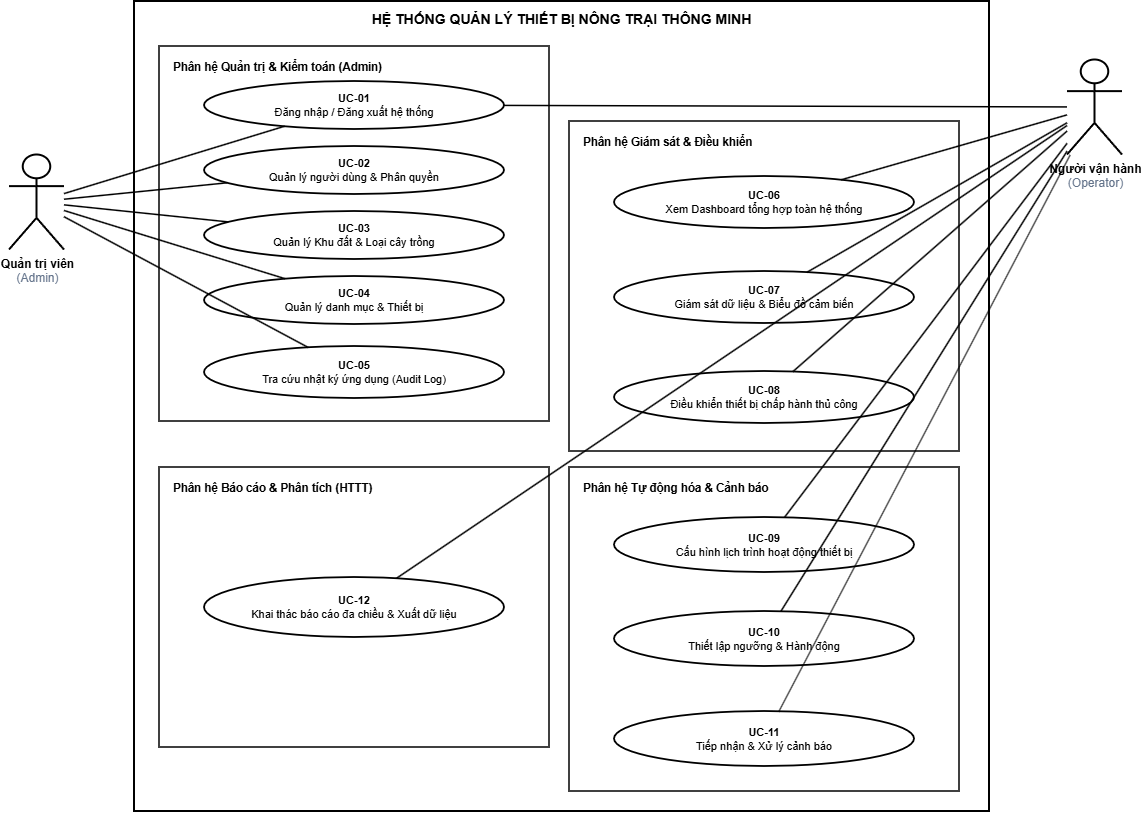
\includegraphics[width=1\textwidth]{images/usecase_diagram.png}
    \caption{Sơ đồ Use Case tổng thể Hệ thống Quản lý Thiết bị Nông trại Thông minh}
    \label{fig:usecase_diagram}
\end{figure}

Sự phân bổ trách nhiệm và quyền hạn truy cập chức năng của các tác nhân được tổng hợp thông qua Ma trận phân nhiệm Use Case tại Bảng~\ref{tab:traceability_matrix}:

\begin{table}[H]
\centering
\small
\begin{tabularx}{\textwidth}{|l|X|>{\centering\arraybackslash}p{2.5cm}|>{\centering\arraybackslash}p{2.5cm}|}
\hline
\textbf{Mã UC} & \textbf{Tên Use Case} & \textbf{Quản trị viên (Admin)} & \textbf{Người vận hành (Operator)} \\ \hline
UC-01 & Đăng nhập / Đăng xuất hệ thống & $\bullet$ & $\bullet$ \\ \hline
UC-02 & Quản lý người dùng \& Phân quyền & $\bullet$ & \\ \hline
UC-03 & Quản lý Khu đất \& Loại cây trồng & $\bullet$ & \\ \hline
UC-04 & Quản lý danh mục \& Thiết bị & $\bullet$ & \\ \hline
UC-05 & Tra cứu nhật ký ứng dụng (Audit Log) & $\bullet$ & \\ \hline
UC-06 & Xem Dashboard tổng hợp toàn hệ thống & $\bullet$ & $\bullet$ \\ \hline
UC-07 & Giám sát dữ liệu \& Biểu đồ cảm biến & & $\bullet$ \\ \hline
UC-08 & Điều khiển thiết bị chấp hành thủ công & & $\bullet$ \\ \hline
UC-09 & Cấu hình lịch trình hoạt động thiết bị & & $\bullet$ \\ \hline
UC-10 & Thiết lập ngưỡng \& Hành động & & $\bullet$ \\ \hline
UC-11 & Tiếp nhận \& Xử lý cảnh báo & & $\bullet$ \\ \hline
UC-12 & Khai thác báo cáo đa chiều \& Xuất dữ liệu & $\bullet$ & $\bullet$ \\ \hline
\end{tabularx}
\caption{Ma trận phân nhiệm vai trò và Use Case trong hệ thống}
\label{tab:traceability_matrix}
\end{table}

\subsection{Đặc tả Use Case chi tiết}

Dưới đây là các bảng đặc tả chi tiết cho các Use Case nghiệp vụ nòng cốt đại diện cho từng phân hệ của hệ thống.

% --- UC-05 ---
\begin{table}[H]
\centering
\small
\begin{tabularx}{\textwidth}{|p{3.2cm}|X|}
\hline
\textbf{Mục} & \textbf{Nội dung đặc tả} \\ \hline
\textbf{Mã Use Case} & \textbf{UC-05} \\ \hline
\textbf{Tên Use Case} & \textbf{Tra cứu nhật ký ứng dụng (Audit Log)} \\ \hline
\textbf{Tác nhân chính} & Quản trị viên (Admin) \\ \hline
\textbf{Mô tả ngắn} & Cho phép Quản trị viên tra cứu, tìm kiếm và thanh tra lịch sử các hành động can thiệp hệ thống của người dùng (đổi ngưỡng, sửa lịch, bật/tắt thủ công). \\ \hline
\textbf{Tiền điều kiện} & Quản trị viên đã đăng nhập thành công vào hệ thống. \\ \hline
\textbf{Hậu điều kiện} & Danh sách các bản ghi nhật ký tương ứng được hiển thị trên giao diện theo đúng tiêu chí tìm kiếm. \\ \hline
\textbf{Luồng sự kiện chính} & 
\begin{enumerate}[leftmargin=*, nosep]
    \item Quản trị viên truy cập vào menu \textit{Quản lý nhật ký ứng dụng}.
    \item Hệ thống hiển thị giao diện bộ lọc gồm: khoảng thời gian, loại hành động, mã nhân viên thao tác và mã thiết bị bị tác động.
    \item Quản trị viên thiết lập các tiêu chí lọc cần tra cứu và nhấn nút \textit{Tìm kiếm}.
    \item Hệ thống truy vấn bảng cơ sở dữ liệu nhật ký nội bộ (Audit Log Table) và hiển thị kết quả phân trang dạng danh sách.
    \item Quản trị viên có thể nhấp chọn từng dòng bản ghi để xem chi tiết thông số cũ và thông số mới được thay đổi.
\end{enumerate} \\ \hline
\textbf{Luồng ngoại lệ} & 
\begin{itemize}[leftmargin=*, nosep]
    \item \textbf{4a. Không tìm thấy kết quả phù hợp:} Hệ thống hiển thị thông báo không có bản ghi nào thỏa mãn điều kiện và hướng dẫn làm mới bộ lọc.
\end{itemize} \\ \hline
\end{tabularx}
\caption{Đặc tả Use Case UC-05: Tra cứu nhật ký ứng dụng (Audit Log)}
\label{tab:uc_05}
\end{table}

% --- UC-08 ---
\begin{table}[H]
\centering
\small
\begin{tabularx}{\textwidth}{|p{3.2cm}|X|}
\hline
\textbf{Mục} & \textbf{Nội dung đặc tả} \\ \hline
\textbf{Mã Use Case} & \textbf{UC-08} \\ \hline
\textbf{Tên Use Case} & \textbf{Điều khiển thiết bị chấp hành thủ công} \\ \hline
\textbf{Tác nhân chính} & Người vận hành (Operator) \\ \hline
\textbf{Mô tả ngắn} & Người vận hành gửi lệnh Bật/Tắt tức thì tới các thiết bị cơ cấu chấp hành (bơm, van tưới, đèn, quạt) từ giao diện Web/App. \\ \hline
\textbf{Tiền điều kiện} & Người dùng đã đăng nhập; thiết bị chấp hành đang ở trạng thái Online và sẵn sàng nhận lệnh. \\ \hline
\textbf{Hậu điều kiện} & Trạng thái hoạt động của thiết bị thay đổi ngoài thực tế; hệ thống tự động lưu một bản ghi tác động vào bảng Audit Log. \\ \hline
\textbf{Luồng sự kiện chính} & 
\begin{enumerate}[leftmargin=*, nosep]
    \item Người vận hành chọn Khu đất và chọn thiết bị chấp hành cần điều khiển.
    \item Người vận hành gạt công tắc Bật/Tắt trên giao diện giám sát.
    \item Hệ thống gửi thông điệp điều khiển xuống thiết bị thông qua giao thức MQTT.
    \item Thiết bị chấp hành thay đổi trạng thái rơ-le và gửi bản tin phản hồi xác nhận (ACK).
    \item Hệ thống cập nhật trạng thái hiển thị mới trên giao diện người dùng.
    \item Hệ thống tự động lưu vết sự kiện điều khiển vào bảng nhật ký ứng dụng (User ID, Device ID, Lệnh điều khiển, Thời gian thực hiện).
\end{enumerate} \\ \hline
\textbf{Luồng ngoại lệ} & 
\begin{itemize}[leftmargin=*, nosep]
    \item \textbf{4a. Quá thời gian phản hồi (Timeout):} Nếu sau 2 giây không nhận được xác nhận từ thiết bị, giao diện khôi phục lại công tắc về trạng thái ban đầu và hiển thị thông báo: \textit{"Không thể kết nối đến thiết bị"}.
\end{itemize} \\ \hline
\end{tabularx}
\caption{Đặc tả Use Case UC-08: Điều khiển thiết bị chấp hành thủ công}
\label{tab:uc_08}
\end{table}

% --- UC-09 ---
\begin{table}[H]
\centering
\small
\begin{tabularx}{\textwidth}{|p{3.2cm}|X|}
\hline
\textbf{Mục} & \textbf{Nội dung đặc tả} \\ \hline
\textbf{Mã Use Case} & \textbf{UC-09} \\ \hline
\textbf{Tên Use Case} & \textbf{Cấu hình lịch trình hoạt động thiết bị} \\ \hline
\textbf{Tác nhân chính} & Người vận hành (Operator) \\ \hline
\textbf{Mô tả ngắn} & Thiết lập lịch trình bật/tắt tự động theo chu kỳ ngày trong tuần và khung giờ trong ngày cho thiết bị chấp hành gắn với từng khu đất và loại cây. \\ \hline
\textbf{Tiền điều kiện} & Người dùng đã xác thực; khu đất, cây trồng và thiết bị đã được cấu hình trên hệ thống. \\ \hline
\textbf{Hậu điều kiện} & Lịch trình mới được lưu trữ và kích hoạt trong tiến trình lập lịch tự động của hệ thống. \\ \hline
\textbf{Luồng sự kiện chính} & 
\begin{enumerate}[leftmargin=*, nosep]
    \item Người vận hành truy cập menu \textit{Quản lý lịch trình}.
    \item Hệ thống hiển thị danh sách các lịch trình hiện hành theo từng Khu đất / Cây trồng.
    \item Người dùng nhấn nút \textit{Tạo lịch trình mới}.
    \item Người dùng chọn Khu đất, chọn thiết bị áp dụng, chu kỳ ngày hoạt động và khung giờ kích hoạt (giờ bật, thời lượng chạy).
    \item Người dùng nhấn nút \textit{Lưu cấu hình}.
    \item Hệ thống kiểm tra tính hợp lệ dữ liệu và kiểm tra xung đột thời gian với các lịch trình đã tồn tại trên thiết bị.
    \item Hệ thống lưu lịch trình vào cơ sở dữ liệu, tự động ghi nhận hành động vào Audit Log và thông báo thành công.
\end{enumerate} \\ \hline
\textbf{Luồng ngoại lệ} & 
\begin{itemize}[leftmargin=*, nosep]
    \item \textbf{6a. Xung đột khung giờ hoạt động:} Nếu thiết bị đã có lịch trình khác chạy trong cùng khoảng thời gian, hệ thống báo lỗi xung đột và yêu cầu người dùng chọn lại thời gian.
    \item \textbf{6b. Bỏ trống trường bắt buộc:} Hệ thống đánh dấu đỏ các trường bị thiếu và yêu cầu người dùng bổ sung đầy đủ.
\end{itemize} \\ \hline
\end{tabularx}
\caption{Đặc tả Use Case UC-09: Cấu hình lịch trình hoạt động thiết bị}
\label{tab:uc_09}
\end{table}

% --- UC-10 ---
\begin{table}[H]
\centering
\small
\begin{tabularx}{\textwidth}{|p{3.2cm}|X|}
\hline
\textbf{Mục} & \textbf{Nội dung đặc tả} \\ \hline
\textbf{Mã Use Case} & \textbf{UC-10} \\ \hline
\textbf{Tên Use Case} & \textbf{Thiết lập ngưỡng \& Hành động} \\ \hline
\textbf{Tác nhân chính} & Người vận hành (Operator) \\ \hline
\textbf{Mô tả ngắn} & Cài đặt dải giá trị môi trường an toàn theo loại cây trồng và cấu hình hành động tự động kích hoạt thiết bị khi phát hiện vi phạm ngưỡng. \\ \hline
\textbf{Tiền điều kiện} & Cảm biến giám sát và thiết bị chấp hành mục tiêu đang hoạt động bình thường trên hệ thống. \\ \hline
\textbf{Hậu điều kiện} & Quy tắc (Rule) được kích hoạt và đưa vào tiến trình kiểm tra dữ liệu chuỗi thời gian của cảm biến. \\ \hline
\textbf{Luồng sự kiện chính} & 
\begin{enumerate}[leftmargin=*, nosep]
    \item Người vận hành truy cập phân hệ \textit{Cài đặt ngưỡng an toàn}.
    \item Chọn Khu đất và Loại cây trồng cần thiết lập.
    \item Nhấn nút \textit{Thêm quy tắc mới}.
    \item Chọn loại cảm biến đo (độ ẩm đất, nhiệt độ) và cài đặt điều kiện biên (ví dụ: Độ ẩm đất $<$ 45\%).
    \item Cấu hình hành động đi kèm (ví dụ: Tự động bật máy bơm tưới trong thời gian 15 phút).
    \item Người dùng nhấn nút \textit{Lưu quy tắc}.
    \item Hệ thống kiểm tra tính hợp lệ số học, lưu quy tắc vào cơ sở dữ liệu, ghi log thao tác và hiển thị thông báo hoàn tất.
\end{enumerate} \\ \hline
\textbf{Luồng ngoại lệ} & 
\begin{itemize}[leftmargin=*, nosep]
    \item \textbf{6a. Ngưỡng số học phi logic:} Nếu người dùng nhập cận dưới lớn hơn cận trên ($Min > Max$), hệ thống báo lỗi và yêu cầu điều chỉnh lại giá trị.
\end{itemize} \\ \hline
\end{tabularx}
\caption{Đặc tả Use Case UC-10: Thiết lập ngưỡng \& Hành động}
\label{tab:uc_10}
\end{table}

% --- UC-11 ---
\begin{table}[H]
\centering
\small
\begin{tabularx}{\textwidth}{|p{3.2cm}|X|}
\hline
\textbf{Mục} & \textbf{Nội dung đặc tả} \\ \hline
\textbf{Mã Use Case} & \textbf{UC-11} \\ \hline
\textbf{Tên Use Case} & \textbf{Tiếp nhận \& Xử lý cảnh báo} \\ \hline
\textbf{Tác nhân chính} & Người vận hành (Operator) \\ \hline
\textbf{Mô tả ngắn} & Hệ thống tự động phát cảnh báo khi số liệu môi trường vượt ngưỡng cho phép; người vận hành tiếp nhận thông báo và ghi nhận kết quả xử lý thực địa. \\ \hline
\textbf{Tiền điều kiện} & Quy tắc ngưỡng (UC-10) đã được kích hoạt; cảm biến đang truyền nhận dữ liệu định kỳ. \\ \hline
\textbf{Hậu điều kiện} & Bản ghi sự cố được lưu trữ; trạng thái cảnh báo chuyển từ \textit{"Đang xử lý"} sang \textit{"Đã giải quyết"}. \\ \hline
\textbf{Luồng sự kiện chính} & 
\begin{enumerate}[leftmargin=*, nosep]
    \item Dữ liệu cảm biến mới gửi về hệ thống vi phạm quy tắc ngưỡng an toàn đã cài đặt.
    \item Hệ thống kích hoạt hành động tự động liên kết (nếu có) và hiển thị thông báo cảnh báo đỏ trên giao diện Dashboard.
    \item Người vận hành nhấp vào biểu tượng cảnh báo để xem thông tin chi tiết (vị trí khu đất, chỉ số đo, thời gian phát hiện).
    \item Người vận hành kiểm tra tình hình thực địa tại nông trại và thực hiện các biện pháp can thiệp cần thiết.
    \item Người vận hành nhấn nút \textit{Xác nhận đã xử lý} trên giao diện và nhập ghi chú khắc phục sự cố.
    \item Hệ thống cập nhật trạng thái sự cố thành \textit{"Đã giải quyết"} và ghi nhận thời gian phản hồi của nhân viên.
\end{enumerate} \\ \hline
\textbf{Luồng ngoại lệ} & 
\begin{itemize}[leftmargin=*, nosep]
    \item \textbf{2a. Kích hoạt hành động tự động thất bại:} Nếu việc tự động bật thiết bị đi kèm không nhận được xác nhận từ rơ-le, hệ thống nâng mức cảnh báo thành \textit{"Khẩn cấp (Critical)"} yêu cầu can thiệp thủ công ngay lập tức.
\end{itemize} \\ \hline
\end{tabularx}
\caption{Đặc tả Use Case UC-11: Tiếp nhận \& Xử lý cảnh báo}
\label{tab:uc_11}
\end{table}

% --- UC-12 ---
\begin{table}[H]
\centering
\small
\begin{tabularx}{\textwidth}{|p{3.2cm}|X|}
\hline
\textbf{Mục} & \textbf{Nội dung đặc tả} \\ \hline
\textbf{Mã Use Case} & \textbf{UC-12} \\ \hline
\textbf{Tên Use Case} & \textbf{Khai thác báo cáo đa chiều \& Xuất dữ liệu} \\ \hline
\textbf{Tác nhân chính} & Người vận hành (Operator), Quản trị viên (Admin) \\ \hline
\textbf{Mô tả ngắn} & Cung cấp công cụ phân tích dữ liệu chuyên biệt của Hệ thống thông tin (HTTT), cho phép lọc dữ liệu đa chiều, trực quan hóa biểu đồ và xuất tệp phục vụ lưu trữ, báo cáo định kỳ. \\ \hline
\textbf{Tiền điều kiện} & Hệ thống đã tích lũy dữ liệu cảm biến và lịch sử vận hành trong cơ sở dữ liệu. \\ \hline
\textbf{Hậu điều kiện} & Báo cáo tổng hợp được hiển thị trên giao diện hoặc tệp dữ liệu được tải về máy tính người dùng. \\ \hline
\textbf{Luồng sự kiện chính} & 
\begin{enumerate}[leftmargin=*, nosep]
    \item Người dùng truy cập phân hệ \textit{Báo cáo \& Phân tích}.
    \item Thiết lập các chiều lọc dữ liệu: Khoảng thời gian (tuần/tháng/vụ mùa), danh sách Khu đất, Loại cây trồng, loại thông số phân tích (nhiệt độ, độ ẩm, thời lượng bơm chạy).
    \item Chọn định dạng hiển thị trực quan (Biểu đồ đường, Biểu đồ cột tổng hợp hoặc Bảng số liệu chi tiết).
    \item Người dùng nhấn nút \textit{Tạo báo cáo}.
    \item Hệ thống thực hiện tính toán tổng hợp dữ liệu (Trung bình, Cực đại, Cực tiểu, Tổng thời gian vận hành) và dựng báo cáo trực quan trên màn hình.
    \item Người dùng chọn định dạng xuất tệp mong muốn (CSV, Excel hoặc PDF) và nhấn nút \textit{Tải xuống}.
    \item Hệ thống đóng gói dữ liệu và tự động tải tệp tin về thiết bị người dùng.
\end{enumerate} \\ \hline
\textbf{Luồng ngoại lệ} & 
\begin{itemize}[leftmargin=*, nosep]
    \item \textbf{5a. Khoảng thời gian không có dữ liệu:} Hệ thống hiển thị thông báo trạng thái rỗng (Empty State) và đề xuất người dùng mở rộng phạm vi thời gian tìm kiếm.
\end{itemize} \\ \hline
\end{tabularx}
\caption{Đặc tả Use Case UC-12: Khai thác báo cáo đa chiều \& Xuất dữ liệu}
\label{tab:uc_12}
\end{table}

% ---------------- TÀI LIỆU THAM KHẢO ----------------
% \pagebreak
% \nocite{*}
% \printbibliography[
%     heading=bibintoc,
%     title={Tài liệu Tham khảo}
% ]

\end{document}